\documentclass[tikz, border=5pt]{standalone}
\usetikzlibrary{arrows.meta, shapes, positioning, automata}

\begin{document}
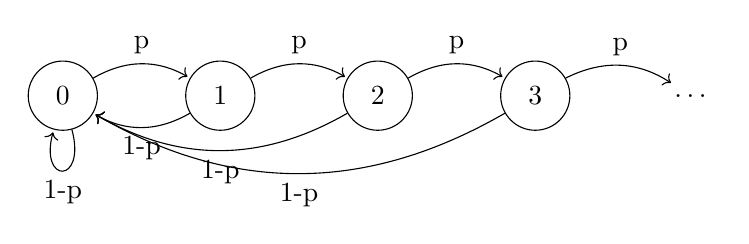
\begin{tikzpicture}[shorten >=1pt, node distance=2cm, on grid, auto]
    % States
    \node[state] (s0) {0};
    \node[state] (s1) [right=of s0] {1};
    \node[state] (s2) [right=of s1] {2};
    \node[state] (s3) [right=of s2] {3};
    \node (dots) [right=of s3] {\ldots};

    % Transitions
    \path[->]
    (s0)
    edge [bend left, above] node {p} (s1)
    edge [loop below] node {1-p} (s0)

    (s1)
    edge [bend left, above] node {p} (s2)
    edge [bend left, below] node {1-p} (s0)

    (s2)
    edge [bend left, above] node {p} (s3)
    edge [bend left, below] node {1-p} (s0)

    (s3)
    edge [bend left, above] node {p} (dots)
    edge [bend left, below] node {1-p} (s0)
    ;
\end{tikzpicture}
\end{document}
